%\begin{abstract}

%\end{abstract}

%\section{keywords}
%\begin{itemize}
%    \item Compare and swap
%    \item Non Blocking Data Structures
%    \item Asynchronous Data Structures
%    \item far memory data structures
%    \item optimisitc concurrency
%
%\section{intro}

% \section{Forward Direction}

% Alex has suggested that I look to the history of these algorithms and then use
% that as a mechanism to discuss what has changed. This is more difficult than
% just reading about dissagregated algorithms.


\section{Introduction}

Disaggregation is an architectural paradigm which separates resources by a
network. While the network provides flexibility, it comes at the cost of latency
-- no where is this more noticeable then the gap between CPU and memory.
Traditionally, access to the memory of a remote machine has be guarded by a CPU
collocated with the memory which can provide serialization service on the
memory, for example an RPC call. Without a remote CPU to serialize all memory
accesses must be coordinated remotely, skyrocketing the cost coordination in the
disaggregated setting.

This high cost coordination environment is not new territory. To reduce
contention overheads in concurrent systems entire classes of lockless data
structures have been produced to reduce contention to only contested regions of
data~\cite{}\todo{add all concurrent structures}. Similarly the advent of NUMA
servers lead to the production of new latency aware algorithms and data
structures which allowed continual
scaling~\cite{linux-scale,black-box-numa}\todo{many cites for numa}. The common
thread that ties these two approaches to the concept of disaggregation is that
memory accesses are one sided, and the latency cost course grained serialization
is high.

These new frontiers are challenging for all involved. It pushes system designers
to carefully design data structures using the lowest synchronization primitives
possible for each task. Further it requires application designers to understand
their application constraints and make intelligent choices for their data
structure usage. While this burden is high, history shows us that it's
achievable~\cite{}~\todo{concurrent linked list, big table, ect} when there is a
lust for scalability and performance.

Disaggregation is still in it's infancy, and it currently lacks the tools and
concepts which will make it accessible to system and application designers.
Foremost is the uncertain architecture of future disaggregated deployments.
Various projects have attempted disaggregated instances, with wide variations in
hardware, from fully custom to
commodity~\cite{dredbox,firebox,machine,legoos}, while little conformity has
been reached in terms of software. These face levels differences make it
difficult even for researchers to determine which problems need to be solved to
achieve practical disaggregation.

In this paper we begin by summarizing prior work on concurrent algorithms, NUMA
algorithms, and RDMA key value stores as many of their techniques lay the
groundwork for disaggregated systems. Then we highlight what makes
disaggregation unique in contrast to this prior work and underscore aspects
which have and have not been addressed. Finally we analyse the first few current
works on disaggregation specific algorithms and analyse their approaches using
our criteria to evaluate the completeness of their solutions.


\section{What this paper is not}

This paper is not an overview of existing disaggregated systems, it's a focus on
the data structures which allow for efficient use of remote memory. Many systems
exist which match the disaggregated model none of which will be covered in
detail. An overview of many of the dissagregated systems which are not covered
here can be found in Yelam et.al~\cite{how-to-build}.

Firstly this is not a paper covering remote paging or caching
systems~\cite{fastswap,kona,infiniswap,leap,legoos}. Each of these has a local
data structure for managing a virtual memory interface.  However none share data
across processes so their only performance effect from far memory is the size of
their cache, paging policy, and round trip time. As such each system is
primarily constrained by the access pattern of their programs. We consider
locality optimization to be a single facet of the design space for
disaggregation and address it more fundamentally in
Section~\ref{sec:techniques}.

% Disaggregated algorithms have the trait that they are one sided, and computed
% over a network.  All shared memory algorithms are one sided, but few are
% designed to scale for hundreds of cores. Often this leads to bottlenecks around
% shared objects such as locks~\cite{linux-scale}. Any shared memory algorithm or
% technique designed to scale is likely applicable to the disaggregated space.

% Therefore the starting place for the history of this exam is concurrency
% algorithms. NUMA systems take care to address the asymmetry of memory accesses
% and divide operations into local and remote. This asymmetry exists in the
% disaggregated context as well. However rather than any piece of data having a
% \textit{local} master, all true data is remote. NUMA systems which allow
% multiple remote accesses to the same data share this quality, and thus their
% techniques are applicable. NUMA which defers to a local core for remote requests
% does not apply here.

\subsection{Lock Free Data Structures}


\subsection{NUMA}

\textbf{Flat Combining~\cite{flat-combine}} Locks and CAS are expensive in their
own right, when highly contested the real cost of using either mechanism can
skyrocket as cache protocols, and fairness skew can dominate access costs and
inflate tail latencies. Flat combining in a technique similar to message
passing, dynamically creates a leader for each access to a critical section. The
leader performs the work of all concurrent requesters in a serialized fashion
and notifies them upon completion. This technique is extremely powerful and is
used in NUMA algorithms~\cite{black-box-numa} as well as RDMA~\cite{flock}. The
key insight here is that the expense of a critical section can be amortized
significantly if is executed within the local confines of a leader, this
simultaneously allows for batching. Individual cores may not be able to push the
request limit of RDMA (7 cores for 8byte 120MOPS on CX5), however on
any particular algorithm they may. In these cases batching will improve
performance. For instance Clover~\cite{clover} would have benefited from flat
combining the requests of local threads, a benefit that Sherman takes complete
advantage of~\cite{sherman}.


\textbf{Partitioned and replicated state}

Shared state is a serious bottleneck for highly parallel systems especially when
the cost of accessing a resource is high. One common pattern is to simply
partition resources so that no sharing is required. For instance systems like
LegoOS~\cite{legoos} and FastSwap~\cite{fastswap} don't support any state
sharing between processes. In multithreaded programs sharing is often an
unavoidable consequence of the work being done. For higher performance processes
can replicate parts of the shared structure and cache the portion locally. In
the case where there is little or no contention this allows processes to make
forward progress without accessing a shared resource. In the disaggregated
setting this is particular important as the cost of accessing remote memory is
particularly high. For instance Clover~\cite{clover} locally caches the metadata
of it's remote database to perform opportunistic writes, and Black Box
Numa~\cite{black-box-numa} maintains a replicated log of every operation. Of
course, when conflicts do occur the benefits of replicating state diminish and
simply become a memory overhead. The choice of replication strategy, and degree
of replication which will result in the highest cost to performance boost is
workload dependent.

\todo{this portion}

\subsection{RDMA}

Why use RDMA? There are a variety of ways to manipulate remote memory,
GMS~\cite{gms} would suggest that we coordinate using full networking stack,
however in the context of disaggregation we assume no remote CPU's to execute
the stack. We could connect via a cache coherent interconnect such a
Kona~\cite{kona} which makes use of cache lines. RDMA is a middle ground. The
RDMA spec gives a set of \textit{verbs} which are memory operations that the NIC
can execute. These verbs are similar in some respects to RPC calls, or simple
instructions. As long as an algorithm can be described using the RDMA calls it
can be executed on remote memory. The advantage to RDMA is that the operations
it supports are general. The downside is that some algorithms are difficult to
execute using one sided verbs. The prototypical example is pointer chasing
which requires a round trip for each resolved pointer.


\subsection{key value stores} 
%% %
The closest space to resource disaggregation is RDMA accelerated key value
stores. In this discipline the expectations of performance have been pushed to
the absolute limit with many projects approaching the latency and throughput of
raw RDMA. These works make careful selection of data structures for efficient
integration with RDMA~\cite{hopscotch,cuckoo}, and select communication
protocols for RDMA which promote the highest performance the current generation
of hardware can offer~\cite{herd,storm}. The direct applicability of prior
KV-store work and disaggregation end when two sided approaches like RPC or two
sided RDMA are utilized for serialization. For example, a common paradigms is to
have the reads be performed async using one sided operations, while the writes
are serialized by a two sided operation~\cite{pilaf}. This allows a CPU to
perform the locking and execute multi step critical sections, such as pointer
chasing, with low latency.

\textbf{Pilaf~\cite{pilaf}} uses just such a mixture of one and two sided RDMA
operations. The key insight is that if a data structure is architects carefully,
the reads can be performed fully asynchronously by one sided RDMA reads which
dramatically reduces server side CPU usage and request latency. This technique
is common in concurrent algorithms, and is readily applicable here. One new
technique for remote memory structures which pilaf introduces is self verifying
data entries. These entries prevent data corruption during races. Incomplete
writes read by RDMA operations can be invalidated by the client. This is one
example of pushing the complexity of a data structure to the client side. Pilaf
does not extend to the disaggregated context directly as writes are handled by a
server side cpu which serializes requests, and processes CRC's. Their rational
is that client side atomic operations are slow, and brittle. 

\textbf{Farm~\cite{farm}}, similar to pilaf allows for async RDMA reads, and
uses one sided writes. However the writes are made to a buffer which is polled
by a server side CPU and later processed as a transaction. This technique in
some ways is a disaggregation applicable approach. At least the writes side of
the rx wheel uses disaggregated techniques. However as half of it's structures
manipulation requires server side processing it is not directly applicable. The
hash table Farm uses is applicable. They use Hopscotch Hashing~\cite{hopscotch}
which places data near keys. This allows a single read to get the values it
needs with a single round trip (as opposed to cuckoo hashing). This pushes the
complexity to the client. To my knowledge this if the first instance of pushing
read complexity to the client in any paper.

\textbf{Herd~\cite{herd}} Herd improves upon both Farm and pilaf by looking
closely at the RDMA specific behavior of KV stores. It considers the hash
algorithm carefully to bound the number of one sided reads. And uses RDMA writes
from server, rather than two sided operations to improve latency. Herds biggest
contribution is that it closely analyses RDMA performance and choses the verb
architecture closely. Herd does not apply greatly to disaggregated contexts as
is fully assumes server side CPUs. However, it's one sided benchmarks are valid
and valuable for disaggregated designers.

\textbf{fasst~\cite{faast}[\textcolor{red}{x}]} Fasst is Anujs first cut at RPC.
Similar to ERPC below, FASST argues heavily for the use of two sided verbs to
reduce the cost of reading. While this makes sense it's not super applicable.
Many of the observations are around batching, RDMA reliability, and scheduling.

\textbf{erpc~\cite{erpc}[\textcolor{red}{x}]} Erpc focues on common case RPC
operations, aiming to reduce drops, avoid pfc, and achieve 100MOPS. This is
almost entirely RDMA optimization. They note that using connections, the
scalability suffers. Around 4000 connections the read rate starts to drop.
Unfortunatly many of the implements for scaling such ad the RPC credit system
rely on server side participation. ERPC is therefore not a good source of info
for this RE.


\textbf{storm~\cite{storm}} Storm makes the argument that modern NICs have the
ability to scale well, in contrast to what has been stated in prior work.

\textbf{1RMA~\cite{1rma}}

Reading through the 1RMA paper~\cite{1rma}, they make the case for basically
using the NIC to execute remote operations and nothing else. In some respects I
def get this aspect of the RDMA construction. Push all of the connection
management to the client side, and just let the RDMA do it's thing with the
extremely high assumption that the packets are going to make it back with a
response. By managing everything on the client side we can get things like
control flow windows, ordering ect without pushing any of this to the hardware
itself. I think that this set of features is somewhat desirable. It would be
cool if the NICs could basically just work on ethernet packets, and then if we
wanted we could interpose on the application level info whenever we wanted.


%currently just a jotting area for ideas.
\section{Remote Memory Techniques}
\label{sec:techniques}

The following are some far/disaggregated memory algorithm design techniques and
common issues.

\subsection{Steering} 
\label{sec:steering}
%
centralized in network compute can be used to steer and modify
requests when data races and conflicts occur. The downside is that this takes an
extra bit of in network processing, but it gets a big speed up. In order for a
middlebox to make the correct steering decision it requires all of the
information necessary to preserve the data invariants of the structure it is
steering into. This limitation demands that the data structure itself be well
conditioned for this property, and be able to deal with potential variance in
its structure.

A potential use for steering is also to perform in place updates while allowing
for reads. For example imagine updating a range on a data structure [x,y] the
first step of the operation could be to lock the region, then copy [x,y] to a
new location [x',y']. During the update reads are steered to the new [x',y'] and
the update is made in place on the old [x,y]. When the operation is complete the
steering stops and the update is atomically visible. This could be useful for
non-pointer based structures like hopscotch hashes~\cite{hopscotch}.

\subsection{Read Size} 
\label{sec:readsize}
%%
One tradeoff that can be made to accelerate writes is to make
them sloppy and push the complexity to the read. This adds a bit of computation
as the reader must compose the information they require from the unsorted read.
As a simple example imagine a multi processes sorted list. Each insert is
expensive if it must be globally coordinated. However it's cheap if each process
just maintains it's own locally sorted list. A call to \textit{max} which
returns the max globally could peek at the heads of each list, and then locally
compute the max from those. For $n$ processes this inflates the cost of the read
by $n$ in bandwidth however it removes the need for coordination. In general I
believe that this holds for all algorithms and data structures. Consider that any
structure can be represented by the set of operations performed on it. If each
write operation is append to a log in memory, with a globally orderable
timestamp then an arbitrary number of processes can have unorganized and full
write throughput, and push the composition of the data structure to each read,
where the entire log of each process is read, and executed locally in it's
entirety.

Algorithms like hopscotch hashing~\cite{hopscotch} (used in Farm~\cite{farm})
and Robinson hashing~\cite{robinhood} are designed to have good cache locality.
They are designed with an open addressing (closed hashing) scheme which states
that an index does not specify the location of the value. However, with these
hashes it will specify the neighborhood of the data, and provide good locality.
If this locality is designed to place relevant information in sequential memory
a scaled up read is appropriate to gain all meta, and data for the structure.
Perhaps more data structures, designed to be concurrent and cache optimized will
be good candidates for Disaggregated Memory.

\subsection{Write amplification mitigation}
\label{sec:write-amplification}
%%
Remote structures sometimes require write
amplification. Consider a set of entries each guarded with a checksum for
integrity. An update to any entry requires the recomputation of the checksum,
and the rewrite of the continuous addresses in order to make the write in a
single round trip. Depending on the bucket size of the entries the write can
grow arbitrarily. Another technique is to make each entry have it's own checksum
for it's integrity, and to only update the bucket checksum when all items become
static.

\subsection{Relaxed Data Layout} Datastructures with struct semantics such as
ordering are difficult to maintain under contention as potentially many elements
must be read, and organized to achieve an operation such as an insert. For
example Sherman~\cite{sherman} uses relaxed ordering in it's B-tree buckets so
that writes can succeed more frequently. Similarly
One-Sided-Hash~\cite{one-sided-hash} uses associative cashing and power of two
in order to allow for multiple write locations. By relaxing the structural
invariants higher write performance is achieved. However this comes at the cost
of read inflation~\ref{sec:readsize} as the correct results must be composed
from an unorganized read. In the case of sherman, relaxing the structure has the
effect of reducing write amplification.

\subsection{Precomputation} Some optimization are easy with preoccupation. Consider
Clio's one level page table~\cite{clio}. Normally a walk would be required, however they
access the page with an O(1) hash. To do so they must avoid collisions. They
push the complexity to malloc which tries continuously to make an virtual address
allocation until it finds one without a hash collision.

\subsection{Optimistic Concurrency} Round trip times are extremely expensive.
Traditional locking requires a round trip for acquisition and for release making
the common case slow. Most far memory algorithms will benefit from optimistic
concurrency with the exception of write heavy ones which must access shared
data. I.e contentious algorithms. RDMA provides verbs such as CAS and FAA for
implementing optimistic concurrency.

\subsection{Memory Traffic} As noted during Yizhous research exam. There is a
potential for a massive amount of additional traffic to flow over the network
due to accessing memory. There are various factors for this. In paging and cache
based transparent systems~\cite{fastswap,kona,gms,infiniswap,legoos,lite}, the
size and associativity of the local cache determines the traffic rate. Each
traffic rate is also a function of the programs memory access policy, and the
systems eviction policy. Shrinking a local cache could significantly inflate
traffic. This is simultaneously true for any cache coherence protocol, or data
structure which needs to have a locally up to date version of remote data prior
to making an update. Memory traffic can be deflated by using traffic agnostic
techniques such as compression, or by modifying the access policy, such as
prefetching more or less remote memory. There is no magic bullet for this
problem, each instance of a remote memory system will have to solve this problem
in its own way.

One aspect of caching protocols is that they explode the traffic requirements.
On memory busses only intended for memory traffic, this may be acceptable, but
on an RDMA network it's going to be most of the traffic. For example the
proposals in Thinking outside of the Box~\cite{design-far-memory-struct} calls
for cache coherence protocols, while Mind~\cite{mind} actually implements one.
Swordbox actually removes the need for the cache coherence by fixing the missing
data in network.

\subsection{Client Side Optimizations}

If clients to remote memory are colocated on the same machine local memory can
be used to consolidate conflicts. For example, designating a single core to make
requests reduces the number of conflicts at remote
memory~\cite{flat-combine}~\cite{sherman}. Many disaggregated solutions supposed
rack scale deployment, therefore while structures must accommodate thousands of
threads, requests can be consolidated at the machine or NUMA level, to reduce
round trips caused by failed contended access to remote locations. This
consolidation requires careful consideration. For example funneling all requests
through a single core will result in a bottle neck. Therefore all non-blocking
operations should be made independently. However, locking operations, if
infrequent could see large performance boosts from client side consolidation.

Properties such as fairness are more easily enforced at the client side. For
example queues are simple. This can allow for cluster approximate fairness where
each machine, or numa domain is fair with respect to itself, but not the system
as a whole.

\subsection{Caching} A variety of caching techniques reduce latency for far memory
application. Caching allows for a two fold benefit. The first is that the
distance between requests and the required data is less. Caching on a switch
removes the last hop in a rack, and on a NIC removes a PCIe round trip. The
dangers with caching is that the important caching data must be determined
somehow. Traditional caching techniques can lead to massive bandwidth inflation.
The second advantage of caching in network is centralization which can reduce
the communication between hosts.


\subsubsection{MIND~\cite{mind}}

Mind uses a programmable switch as a memory controller. It tracks access to
memory regions using a centralized cache. It makes use of the MSI cache
coherence protocol (Modified, Shared, Invalid) which essentially acts as
read/write locks on the memory. Shared means that many processes can read shared
memory, modified means that it's dirty and owned by a single process, invalid
means it's not present. Mind provides both memory protection and cache
coherence. It's not going to be able to compete with
SwordBox~\cite{Grant2021InContRes} as it is blocking.

\section{remote memory traps}

\textbf{Centralized Serialization} My approach uses a centralized serialization
point to alleviate coordination. However it has been shown that doing all the
work by a centralized core is slower than a carefully crafted concurrent
solution~\cite{near-memory-structs}. The insight here is that if we have a core
close to memory it can do things like pointer chasing faster than remote. They
demonstrate that PIMs are not sufficient to solve far memory problems. But it
will become bogged down at some point due to being centralized. That's when a
concurrent algorithm with less contention moves faster. The key thing about this
centralized point, is that it must have excess space above line rate with which
to coordinate. For example in ~\cite{fairnic}[Figure 2] we show that there is
some headroom for processing with x number of cores. This gap is the processing
gap that we can use to resolve contention.

\textbf{RDMA Atomics} Relying on RDMA atomics may lead a design to reach
artificial bottlenecks. RDMA atomics perform at roughly half the rate of
identically sized writes. For example Clover~\cite{clover} under extreme
contention would suffer from the CAS bottleneck. Almost every remote structure
uses CAS to some extent~\todo{Breif Summary of CAS papers}. Papers such as
Sherman~\cite{sherman} have noted that they can get better single location CAS
and FFA performance by utilizing device mapped memory. This is a nice
performance improvement, but it's still comparatively slow by my own
measurements.

CAS operations are slightly faster than FAA by my measurements when contested.
They can be used in concert to achieve differing levels of performance with
different semantics. For example CAS to lock, and FAA to unlock.

RDMA locks lack fairness. Using existing CAS and FAA locking there is not a
reasonable way to achieve fair locking with low round trip times. Thus any RDMA
concurrent structure leveraging CAS locks will potentially lead to starvation
and high tail latency.

\textbf{Round Trip Locks}

Local serialized locking scales poorly to disaggregation. Acquiring a lock,
performing work, and then unlocking, is not expensive when memory is only a few
nanoseconds away, but when each operation represents a round trip its cost
skyrockets. The common approach takes 4 round trips. The first to acquire the
lock, the second to read the required data, another to write an update, and a
final message to unlock. Amortizing this cost is key in disaggregation. Using
common concurrency patterns the cost can be reduced. For instance it can be
reduced to 3 by performing the read first, then the write, and then
opportunistically attempting a lock which commits the write. Typically this will
fail if the read was stale, or another thread move the data structure forward
concurrently. This can be further improved by amortizing the reads and writes.
For instance reads can be done out of band with writes to attempt and keep a
local cache up to date. On writes, the write is performed simultaneously with
the opportunistic lock. In the best case this reduces the observed latency on a
write to a single round trip, but it can easily degrade to many retires if write
or read data is contested. Clover~\cite{clover} Caches metadata locally and
performs reads of the metadata out of band. Writes require two round trips, the
first to perform the write to a processes isolated location, and a second to
link the write to a shared data structure using an RDMA CAS operation.

\section{Disaggregated Algorithms}

\subsection{Clover}

\subsection{Write Conscious Hashing}

\subsection{Sherman Btree}

Optimizations - Local Caching of locks. Use of In-order delivery RDMA to
coalesce writes. Unsorted B-Tree leaves. On NIC memory locks.

Client side optimizations. A technique like flat combining is used for local
locks~\cite{flat-combine}, whenever possible client side locking is used, and
requests are issued by a centralized client side arbiter. Data structure layout
is RDMA optimized. Sherman is truly write optimized. When writes occur they are
unordered on their leaf nodes to prevent write amplification and the need to
retry. Reads are totally async and use entry level version numbers to validate
themselves. Lookups can fail frequently, and the remedy is to retry. For
instance overlapping reads and writes will lead to a retry. Range query are
complex in that they do no contain consistent values. For transactional reads to
occur reads must also lock. This is a strict lessening of constancy which may
not be desireable for future applications.

\subsection{Ford}

\section{Middlebox Incorporation}

The increased gap between computational resources and memory in the
disaggregated model leads to poor performance in some cases. The most blatant is
serialization on contended resources. As noted in Sherman, Clover, Conscious
Hashing~\cite{sherman,clover,one-sided-hash}, writes must be carefully
coordinated to avoid collisions. Fast serialization can be achieved using a
centralized source such as programable hardware in the network. This hardware
performs serialization at the physical level, and is able to process millions of
requests per second. Netlock~\cite{netlock} demonstrates that a switch can
provide centralized locking for millions of requests per second. Mind,
demonstrates that memory protection and cache coherence can be maintained by a
switch~\cite{mind}, and NetChain demonstrated that a set of switches can be used
to obtain millions of consensus operations per second. There are countless works
on in network acceleration for a variety of tasks~\todo{ipipe,netcache,itterally all the things}.

Including a middlebox into the architectural design of a disaggregated system is
a common pattern~\cite{disandapp}. In this model a centralized network device
provides some memory services to the application such as memory protection. The
performance benefit from serialization makes network devices tempting as a key
component of disaggregated systems especially with the proliferation of
programmable networking platforms such as Barefoot Tofino~\cite{tofino3} and
Corundum~\cite{corundum} make developing such software more accessible than ever.

However there is a sweet spot in terms of utility with programable network
devices, Figure~\ref{fig:middlebox_model} shows a general model for network hardware
performance as it does more work per packet. If the work necessary from a
middlebox is higher than a specific number of cycles per packet, then the
overall performance drops below the beneficial range. It has been show in
simulations for PIM architectures that a centralized serialization point for
operations like pointer chasing can slow down operations compared to well
designed data structures for concurrency~\todo{pim Irina citation}.

Therefore the choice of network computation is a balancing act for resource
disaggregation. The balancing act is not only in the choice of \textit{what?}
computation to perform in network, but how the computation should be structured.
Deferring all locking operations to a switch for instance dominates it's spare
resources. If the algorithm making use of switch implemented locks could instead
be implemented using a concurrent algorithm which only makes use of CAS
operations. This would be a fine candidate for RDMA primitives which could
alleviate resource pressure on the switch.

This principle leads to a very simple design guideline for memory
disaggregation. \textbf{Implement all far memory structures with the fewest
constraints possible}. End-to-end approaches should be able to achieve their
operations in O(1) in the common case as round trips are the greatest enemy of
performance.  Clients will benefit from caching data, and performing additional
computation rather than making additional remote requests. Examples include
relaxing data structure invariants such as ordering and placement. Further
networks are fast, and have high bandwidths, if necessary performing larger
reads to obtain correct data is a better decision than making many round trips
to perform a write. If data is truly contested i.e locks, and hot keys,
\textbf{middleboxes such as switches and NICs can provide fast serialization}.
Less is more when leveraging a network device. Algorithms and data structures
leveraging middlebox should be specially tuned to reduce middlebox state. Ideal
data structures would have structural invariants which a middlebox can maintain
while only keeping a small fraction of the data structures information in
memory. Lastly the work done by the middlebox should be minimal. Complex
operations are not ideal for hardware designed to forward packets. Algorithms
with operations that can be satisfied by swapping out values in packets are
ideal. As an example changing the location of a read or write, changing the side
of a read or write, or setting a value in the packets payload. As demonstrated
in SwordBox~\cite{Grant2021InContRes} contention can be avoided in append only
link lists by caching the location of the tail of the list.

\begin{figure}
    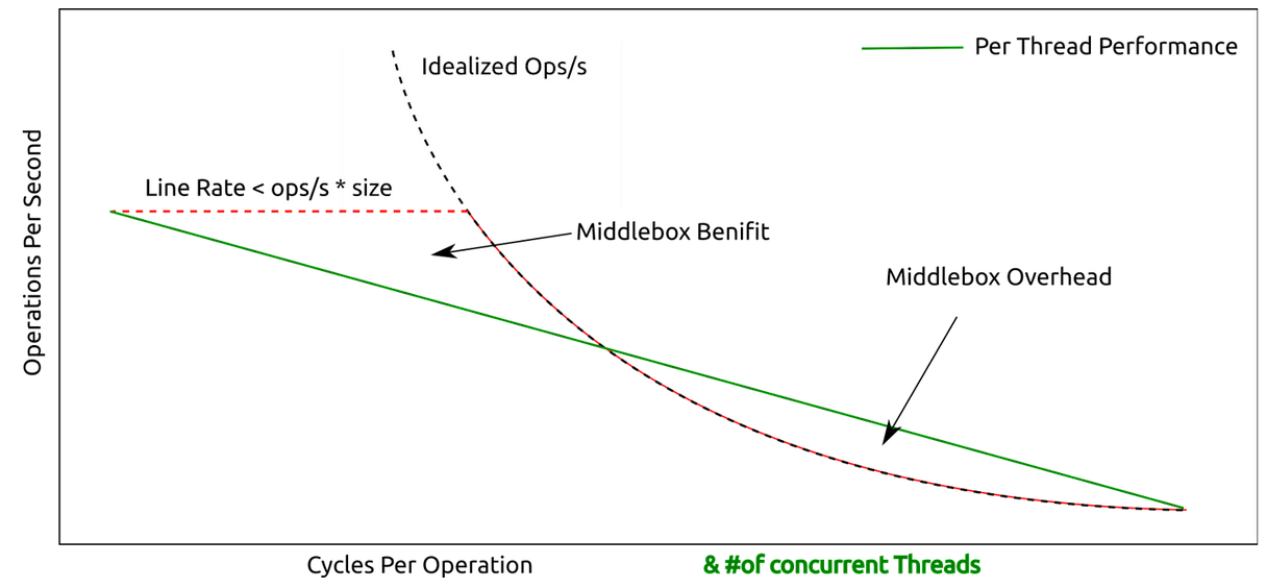
\includegraphics[width=0.45\textwidth]{fig/middlebox_model.png}

    \caption{Middlebox only support a bounded number of cycles per operation
    before their performance drops below line rate. A programs performance can
    only benefit from middlebox intervention if it's requirements per operation
    fall below this threshold.}

    \label{fig:middlebox_model}
\end{figure}

\subsection{Mind}



\section{notes}

The papers~\cite{one-sided-hash} and ~\cite{write-optimized-hash} are almost
identical. It's the same author, I'm just noting that the change between NUMA
and Far memory could use this as a case study.

Similar to the concept of a bandwidth delay product, in terms of remote memory
there is a latency operation product which is expanded by the time it takes for
an operation to complete. For example O(1) will have less active operations than
an O(2) data structure simply by the nature of the operations. Anything requiring
a read and a write to complete will take longer to complete due to the round
trip.

In the few concurrent papers I read there is the concept of performing a marking
on a data structure. For example this concurrent binary
tree~\cite{fast-concurrent-bin} marks edges to ensure that they do not get
modified in a way that breaks the tree. This marking is similar to placing a
lock. I think that similar to marking, there should be a way to check a data
structures in flight operations, if all the operations are known ahead of time,
and then serialize the requests based on that.

There is a good argument for algorithms between the two worlds of remote memory.
On one hand we have pure remote memory, one sided operations with zero
interference. These are unbelievably slow. And we can say from a straw man
perspective that they could use better algorithms. On the other hand we have
solutions like in~\cite{design-far-memory-struct,near-memory-structs}, which
suggest near memory computing with on board compute near memory. In this case
they also show that with the best near memory compute the old algorithms simply
do not work because the serialization gets overloaded.

Would it be possible to implement transactional memory on a switch? How far off
is Mind~\cite{mind} from doing this?

\section{Figures}




%\section{review}  

%\section{conclusion}